\documentclass[hyperref,]{ctexart}
\usepackage{lmodern}
\usepackage{amssymb,amsmath}
\usepackage{ifxetex,ifluatex}
\usepackage{fixltx2e} % provides \textsubscript
\ifnum 0\ifxetex 1\fi\ifluatex 1\fi=0 % if pdftex
  \usepackage[T1]{fontenc}
  \usepackage[utf8]{inputenc}
\else % if luatex or xelatex
  \ifxetex
    \usepackage{xltxtra,xunicode}
  \else
    \usepackage{fontspec}
  \fi
  \defaultfontfeatures{Mapping=tex-text,Scale=MatchLowercase}
  \newcommand{\euro}{€}
\fi
% use upquote if available, for straight quotes in verbatim environments
\IfFileExists{upquote.sty}{\usepackage{upquote}}{}
% use microtype if available
\IfFileExists{microtype.sty}{%
\usepackage{microtype}
\UseMicrotypeSet[protrusion]{basicmath} % disable protrusion for tt fonts
}{}
\ifxetex
  \usepackage[setpagesize=false, % page size defined by xetex
              unicode=false, % unicode breaks when used with xetex
              xetex]{hyperref}
\else
  \usepackage[unicode=true]{hyperref}
\fi
\usepackage[usenames,dvipsnames]{color}
\hypersetup{breaklinks=true,
            bookmarks=true,
            pdfauthor={蓝海; 彭莉},
            pdftitle={分析申坤-技术报告},
            colorlinks=true,
            citecolor=blue,
            urlcolor=blue,
            linkcolor=magenta,
            pdfborder={0 0 0}}
\urlstyle{same}  % don't use monospace font for urls
\usepackage{longtable,booktabs}
\usepackage{graphicx,grffile}
\makeatletter
\def\maxwidth{\ifdim\Gin@nat@width>\linewidth\linewidth\else\Gin@nat@width\fi}
\def\maxheight{\ifdim\Gin@nat@height>\textheight\textheight\else\Gin@nat@height\fi}
\makeatother
% Scale images if necessary, so that they will not overflow the page
% margins by default, and it is still possible to overwrite the defaults
% using explicit options in \includegraphics[width, height, ...]{}
\setkeys{Gin}{width=\maxwidth,height=\maxheight,keepaspectratio}
\setlength{\emergencystretch}{3em}  % prevent overfull lines
\providecommand{\tightlist}{%
  \setlength{\itemsep}{0pt}\setlength{\parskip}{0pt}}
\setcounter{secnumdepth}{5}

\title{分析申坤-技术报告}
\author{蓝海 \and 彭莉}
\date{}

% Redefines (sub)paragraphs to behave more like sections
\ifx\paragraph\undefined\else
\let\oldparagraph\paragraph
\renewcommand{\paragraph}[1]{\oldparagraph{#1}\mbox{}}
\fi
\ifx\subparagraph\undefined\else
\let\oldsubparagraph\subparagraph
\renewcommand{\subparagraph}[1]{\oldsubparagraph{#1}\mbox{}}
\fi

\begin{document}
\maketitle

{
\setcounter{tocdepth}{2}
\tableofcontents
}
\section{业绩表现}

\subsection{申坤}

女,硕士研究生。2010年4月加入国泰基金管理有限公司,历任研究员、基金经理助理。2015年6月起任国泰成长优选混合型证券投资基金(原国泰成长优选股票型证券投资基金)的基金经理。

申坤前后共管理过2个不同的基金产品,分别是:国泰金鑫和国泰成长优选混合。

\subsection{当前表现}

\subsubsection{国泰金鑫}

\begin{figure}[htbp]
\centering
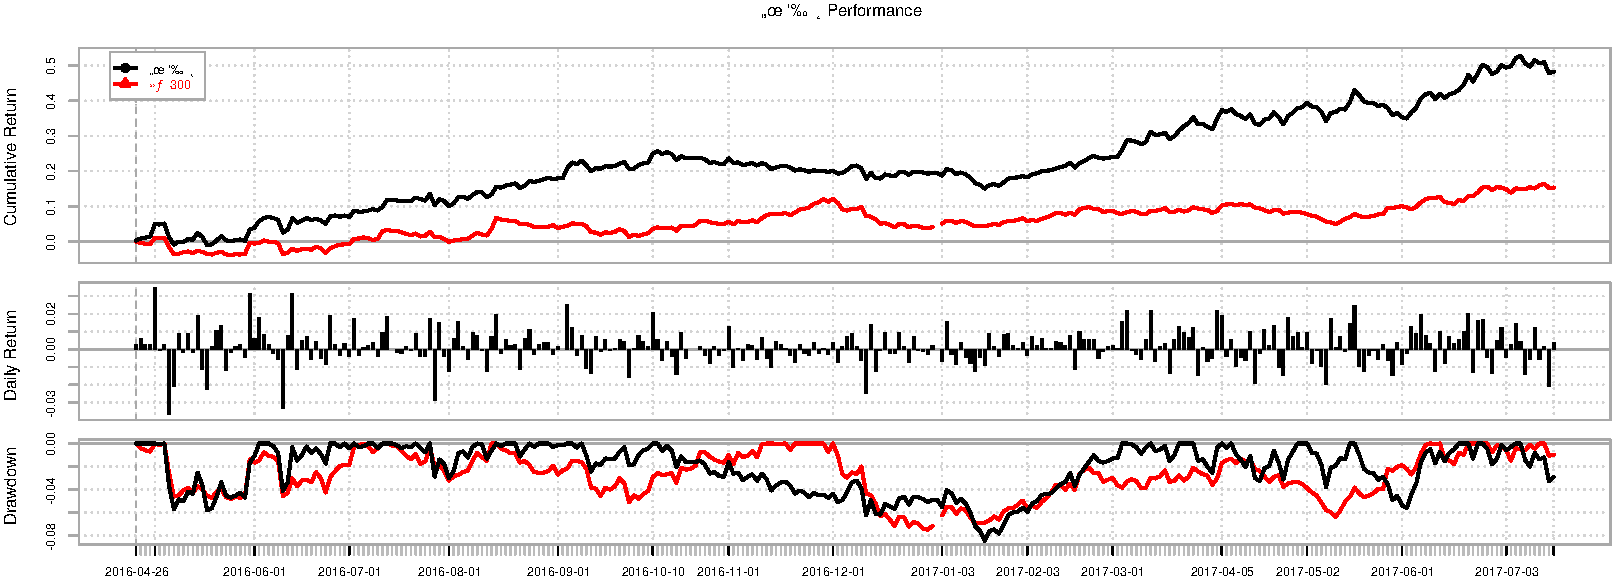
\includegraphics{shenkun-details_files/figure-latex/unnamed-chunk-2-1.pdf}
\caption{基金累计回报率与回撤}
\end{figure}

\begin{longtable}[]{@{}llclclc@{}}
\toprule
名称 & 近半年 & 夏普率 & 近一年 & 夏普率 & 近两年 &
夏普率\tabularnewline
\midrule
\endhead
国泰金鑫 & 23.3\% & 3.0 & 39\% & 2.24 & 48\% & 2.13\tabularnewline
沪深300 & 8.9\% & 1.6 & 16\% & 0.85 & 15\% & 0.73\tabularnewline
\bottomrule
\end{longtable}

\begin{figure}[htbp]
\centering
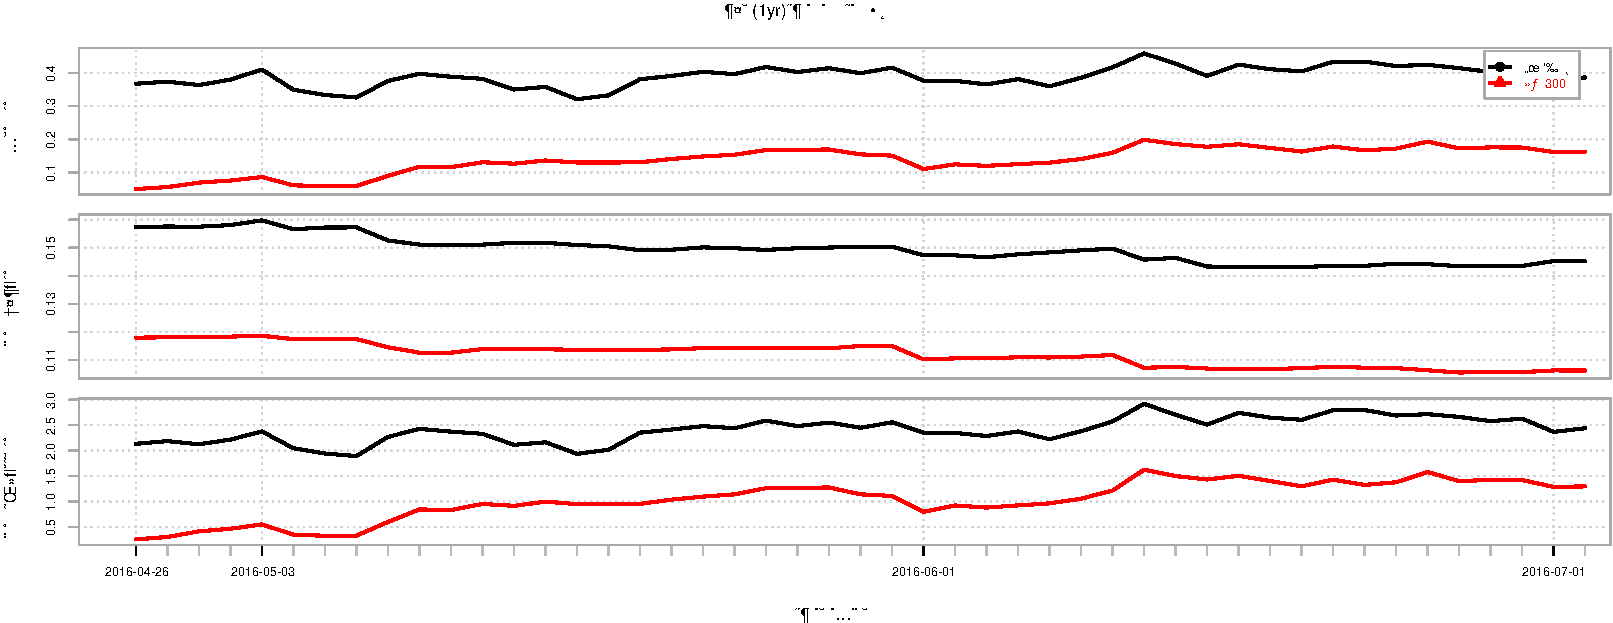
\includegraphics{shenkun-details_files/figure-latex/unnamed-chunk-3-1.pdf}
\caption{投资着收益风险比较}
\end{figure}

图1清楚的表明自申坤在管理该两支基金以来相对于沪深300其累计收益率的不俗表现,尤其是其走势与沪深300的有逆向而行的意思,这对于投资者配置资产组合时是很好的标的。图2明确的表明,固定一年期的投资者,无论何时买入这两只基金,她都可以获得相比沪深300更高的累计收益,虽然面临的波动要高一些,但是日收益序列的风险收益比------夏普率------都是显著高于沪深300的。通俗的说,就是不但能够赚更多的钱,而且作为投资者,你还更有可能``拿得住''这样的投资对象,因为收益波动比更大。当然由于申坤管理这支基金的时间不长,我们能够做出的判断都是基于较短的时间序列上的,只有时间才能验证一切。

\subsubsection{国泰成长优选混合}

\begin{figure}[htbp]
\centering
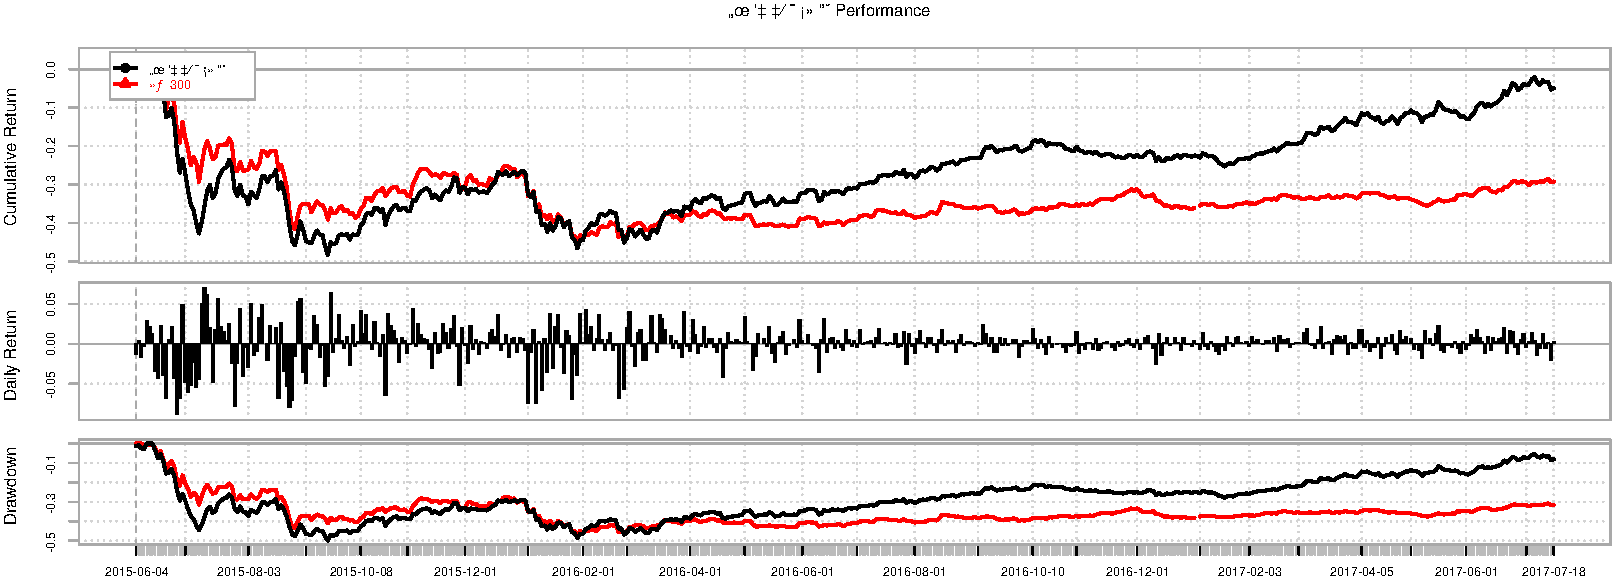
\includegraphics{shenkun-details_files/figure-latex/unnamed-chunk-4-1.pdf}
\caption{基金累计回报率与回撤}
\end{figure}

\begin{longtable}[]{@{}llclclc@{}}
\toprule
名称 & 近半年 & 夏普率 & 近一年 & 夏普率 & 近两年 &
夏普率\tabularnewline
\midrule
\endhead
国泰成长优选混合 & 22.1\% & 3.0 & 38\% & -0.12 & -5\% &
-0.18\tabularnewline
沪深300 & 8.9\% & 1.6 & 16\% & -0.62 & -29\% & -0.66\tabularnewline
\bottomrule
\end{longtable}

由于成长股的特性,在股灾时期其回撤大于沪深300,几乎跌去一半。在2016年2月以后表现非常的抢眼。这与另外以为成长股里的明星经理王培的经历出奇的相似。这当中或许隐藏者一些有趣的东西,在以后我们会专门的分析。
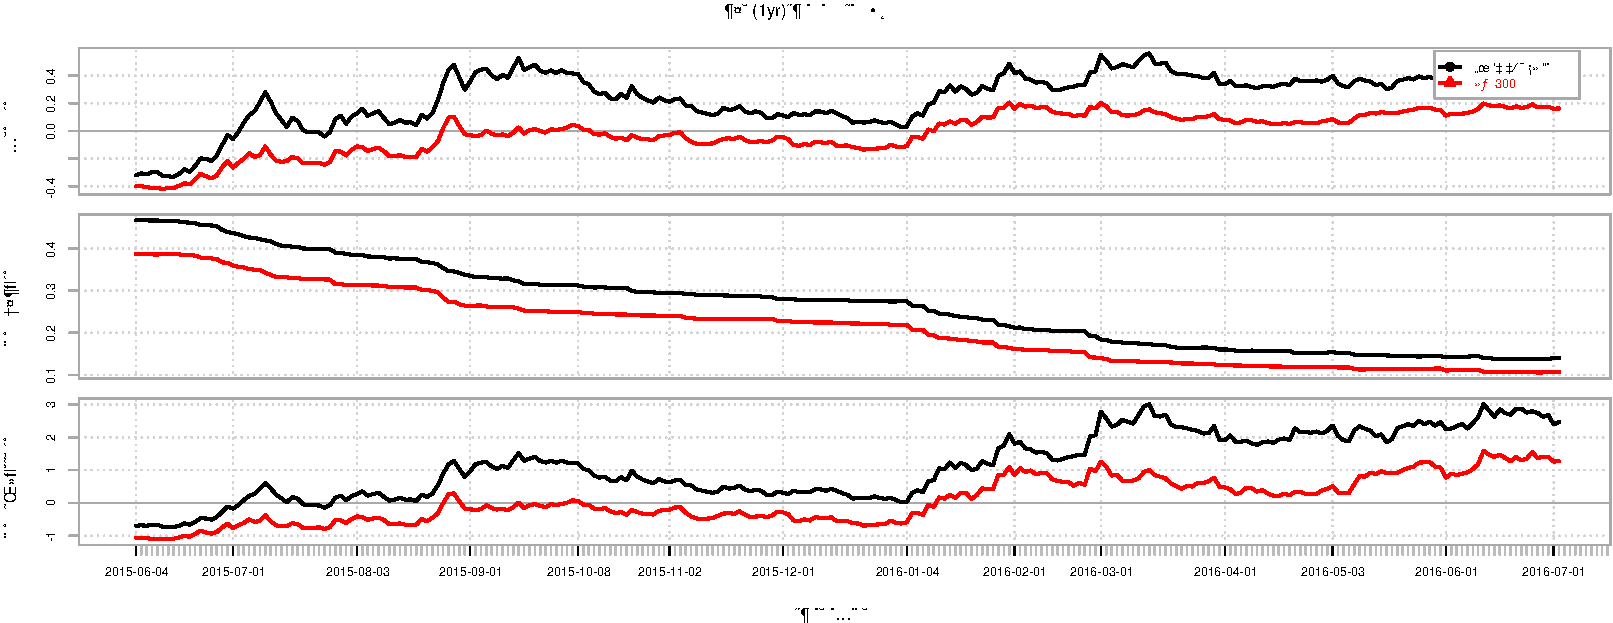
\includegraphics{shenkun-details_files/figure-latex/unnamed-chunk-5-1.pdf}

作为一年期定期投资者选择投资国泰金鑫可定有超过沪深300的表现,但是绝对收益是没有保证的。另外一个值得一提的好处是,尽管波动率大于沪深300,但是其收益波动比还是要好于沪深300。

\section{风格分析}

\subsection{交易风格}

基于公开信息,我们对申坤的正在管理的国泰金鑫的交易风格分析如下:

\begin{longtable}[]{@{}lcccccc@{}}
\toprule
日期 & 换手率 & 排名\% & 持有期 & 排名\% & 前十占比\% &
排名\%\tabularnewline
\midrule
\endhead
2016 Q2 & 242 & 40 & 0.22 & 69 & 55 & 32\tabularnewline
2016 Q4 & 537 & 33 & 0.10 & 76 & 64 & 17\tabularnewline
\bottomrule
\end{longtable}

\begin{longtable}[]{@{}lccccrcrc@{}}
\toprule
日期 & 行业前5占比\% & 排名\% & 平均集中度 & 排名\% & PE & 排名\% & PB &
排名\%\tabularnewline
\midrule
\endhead
2016 Q2 & 100 & 17 & 0.16 & 54 & 30 & 65 & 4.3 & 47\tabularnewline
2016 Q4 & 100 & 15 & 0.17 & 53 & 35 & 42 & 3.9 & 35\tabularnewline
\bottomrule
\end{longtable}

换手率略高而持有期处于中间水准,似乎意味着有一些波段操作,在之后的择时能力中进行验证。前10股票占比较高而行业集中也相当高,用她自己的话说,是``好行业难寻,找到了就重配''。成长股的估值不便宜,所以持股的品均PE和PB都在平均水平之上。从以上表格中可以看出
\emph{申坤,是以适当高的换手率,集中的投资于精选的成长型股票来获取收益的,尤其是行业的集中度很高,她更像是一个主题投资者}。

同样的对于国泰成长优选混合进行交易风格分析,我们也发现了相似的情况。数据如下:

\begin{longtable}[]{@{}lcccccc@{}}
\toprule
日期 & 换手率 & 排名\% & 持有期 & 排名\% & 前十占比\% &
排名\%\tabularnewline
\midrule
\endhead
2015 Q2 & 241 & 64 & 0.19 & 55 & 42 & 87\tabularnewline
2015 Q4 & 564 & 64 & 0.08 & 75 & 55 & 55\tabularnewline
2016 Q2 & 264 & 43 & 0.19 & 71 & 59 & 48\tabularnewline
2016 Q4 & 718 & 29 & 0.07 & 85 & 70 & 34\tabularnewline
\bottomrule
\end{longtable}

\begin{longtable}[]{@{}lccccrcrc@{}}
\toprule
日期 & 行业前5占比\% & 排名\% & 平均集中度 & 排名\% & PE & 排名\% & PB &
排名\%\tabularnewline
\midrule
\endhead
2015 Q2 & 92 & 72 & 0.07 & 78 & 41 & 61 & 6.9 & 43\tabularnewline
2015 Q4 & 99 & 29 & 0.06 & 70 & 44 & 56 & 6.0 & 41\tabularnewline
2016 Q2 & 97 & 49 & 0.04 & 72 & 30 & 61 & 4.4 & 42\tabularnewline
2016 Q4 & 100 & 21 & 0.13 & 36 & 54 & 17 & 3.4 & 36\tabularnewline
\bottomrule
\end{longtable}

需要进一步解释的是为什么行业前五占比高达92\%而在2015年2季度的时候行业排名是靠后的72\%呢。这是因为牛市的时候投资者普遍详细强者恒强,都把投资集中到自己熟悉、有把握的股票上以期在牛市中博得最大收益。

\subsection{持仓风格}

基于净值数据,我们对申坤的持仓风格分析如下。

\subsubsection{国泰金鑫}\label{-1}

\begin{longtable}[]{@{}ccc@{}}
\caption{持仓风格权重分析(\%)}\tabularnewline
\toprule
大盘价值 & 中盘成长 & 货币\tabularnewline
\midrule
\endfirsthead
\toprule
大盘价值 & 中盘成长 & 货币\tabularnewline
\midrule
\endhead
1 & 79 & 20\tabularnewline
\bottomrule
\end{longtable}

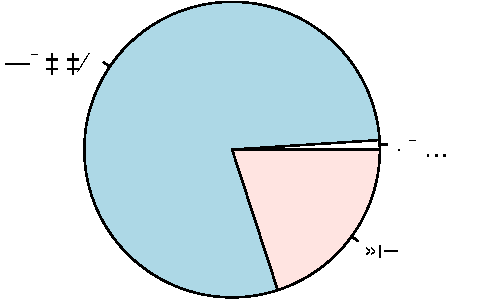
\includegraphics{shenkun-details_files/figure-latex/unnamed-chunk-8-1.pdf}

虽然我们的风格分析是基于净值数据的,但是经过比较持仓数据,结果还是相当准确的。持有约20\%的货币有点奇怪,但是考虑到2016年债券市场的剧烈波动,消费品行业研究员出生的申坤选择宁愿持有货币而不是债券也是情有可原的。

\subsubsection{国泰成长优选混合}\label{-1}

\begin{longtable}[]{@{}cccc@{}}
\caption{持仓风格权重分析(\%)}\tabularnewline
\toprule
大盘价值 & 中盘成长 & 小盘成长 & 货币\tabularnewline
\midrule
\endfirsthead
\toprule
大盘价值 & 中盘成长 & 小盘成长 & 货币\tabularnewline
\midrule
\endhead
2 & 73 & 20 & 5\tabularnewline
\bottomrule
\end{longtable}

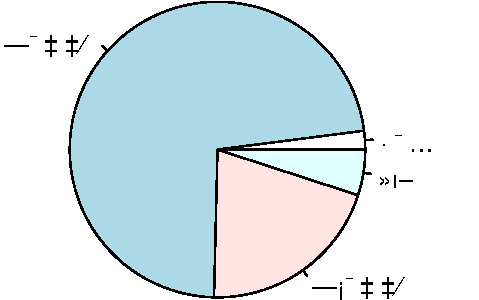
\includegraphics{shenkun-details_files/figure-latex/unnamed-chunk-9-1.pdf}

此模型回归的\(R^2=\)
0.83,不是特别精确,也在可接受范围。其重点投资的股票往往都是成长类型的股票。持有的大盘价值,是上汽集团,大体占净值的弱2\%。

从中可见,\emph{申坤是一个偏爱中等规模的成长类股票的投资者}。

\subsection{主动风格:积极}

我们用行业累计偏离指数代表该基金主动管理的活跃度(在Kacperczyk等的研究中,这个指标又被成为行业集中度)。我们的逻辑根据建立在弱有效市场指数代表了整个市场的``简单''共识,大量的``smart
beta''的机会留给了基金管理人,在追寻``smart
beta''的过程中,突破原有的行业布局不可避免。而这种突破正可以被行业累计偏离指数来捕捉。但是,主动指数并非越大越好,毕竟市场是弱有效的,完全忽略市场的共识------哪怕是``简单''共识------也是唐吉坷德式的挑战风车。实际上有研究表明,基金业绩表现与Kacperczyk的行业集中度呈现负相关,即行业集中度越大,基金表现越差。我们的分析表明,这种联系在中国市场不是简单照搬的,对于极端的行业集中的情形,确实行业集中度越高,基金平均表现越差,但是在一个温和的区间中,这样的联系是不存在的。当然这个主动指数可以进一步的拓展到对包含基金经理追求alpha
的描述,这是我们下一步的工作方向之一。

以其管理的国泰成长优选混合基金为说明,从创建到其接收管理之前,该基金的平均主动管理活跃度为35\%,呈现非常积极的主动管理态势;其接管基金后平均主动管理活跃度为32\%,风格延续。在其管理的同期,整个基金行业的同类型基金的主动管理活跃指数为27\%。因此,\emph{对于申坤的管理风格可以定义为积极的主动管理型}。

\section{能力评价}

\subsection{大类资产配置:几乎为零}

从下图可以看出,自从2015年11月接手以来,申坤在产品国泰金鑫中将股票仓位控制在80-90\%之间,而另外一个产品国泰成长优选混合股票仓位则也类似的在70\%-85\%之间变换。

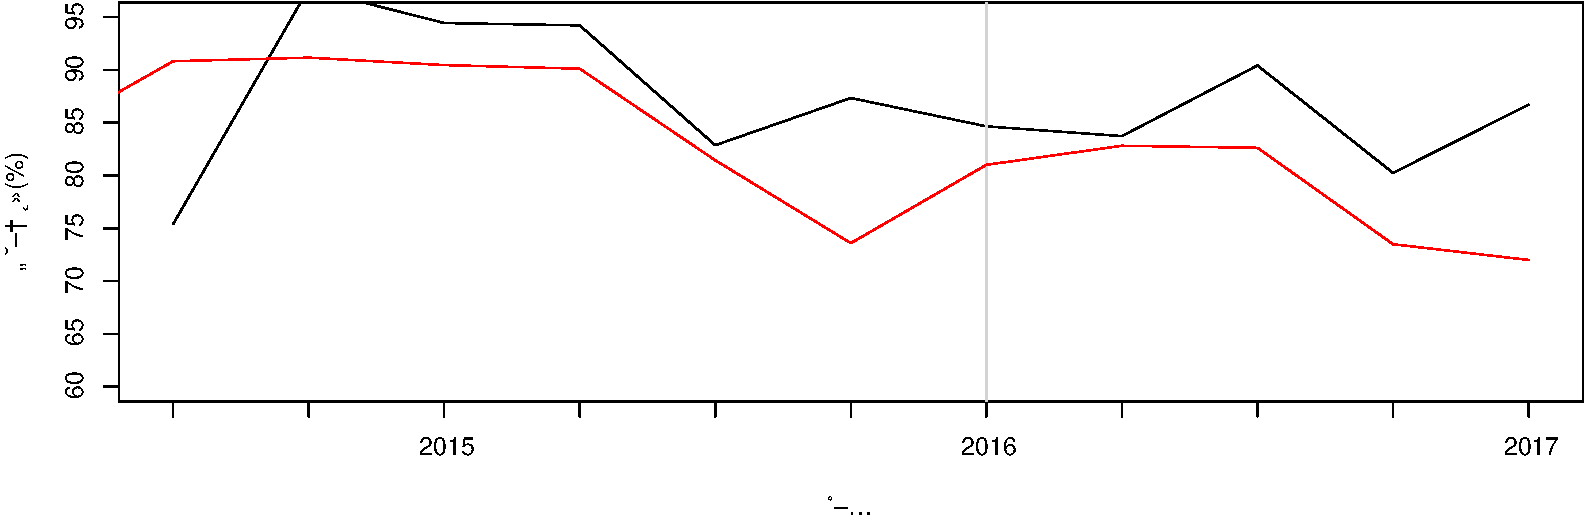
\includegraphics{shenkun-details_files/figure-latex/unnamed-chunk-11-1.pdf}

进一步的计算大类资产配置带来的超额收益。

\subsubsection{国泰金鑫}\label{-2}

\begin{longtable}[]{@{}lc@{}}
\caption{国泰金鑫大类资产配置能力统计}\tabularnewline
\toprule
日期 & 大类资产配置超额贡献(\%)\tabularnewline
\midrule
\endfirsthead
\toprule
日期 & 大类资产配置超额贡献(\%)\tabularnewline
\midrule
\endhead
2016 Q2 & 0.19\tabularnewline
2016 Q3 & -0.18\tabularnewline
2016 Q4 & 0.18\tabularnewline
2017 Q1 & -0.14\tabularnewline
\bottomrule
\end{longtable}

\begin{longtable}[]{@{}cl@{}}
\toprule
平均超额贡献(\%) & 90\%置信区间\tabularnewline
\midrule
\endhead
0.013 & \([-0.15,\infty)\)\tabularnewline
\bottomrule
\end{longtable}

统计显示,在国泰金鑫这支基金的管理上,虽然每季度平均取得 0.01\%
的配置收益,但是统计意义上并不显著。因此申坤并没有显示出大类资产配置的能力。

\subsubsection{国泰成长优选混合}\label{-2}

\begin{longtable}[]{@{}lc@{}}
\caption{国泰金鑫大类资产配置能力统计}\tabularnewline
\toprule
日期 & 大类资产配置超额贡献(\%)\tabularnewline
\midrule
\endfirsthead
\toprule
日期 & 大类资产配置超额贡献(\%)\tabularnewline
\midrule
\endhead
2015 Q2 & 0.7399\tabularnewline
2015 Q3 & -1.8566\tabularnewline
2015 Q4 & -0.6992\tabularnewline
2016 Q1 & 0.3365\tabularnewline
2016 Q2 & 0.0055\tabularnewline
2016 Q3 & -0.1457\tabularnewline
2016 Q4 & 0.4310\tabularnewline
2017 Q1 & -0.0658\tabularnewline
\bottomrule
\end{longtable}

\begin{longtable}[]{@{}cl@{}}
\toprule
平均超额贡献\% & 90\%置信区间\tabularnewline
\midrule
\endhead
-0.16 & \([-0.56,\infty)\)\tabularnewline
\bottomrule
\end{longtable}

统计显示,在中欧潜力价值灵活配置混合这支基金的管理上,每季度平均取得
-0.16\% 的配置收益。因此申坤并没有显示出大类资产配置的能力。

综上,结合仓位控制上的变化以及专项计算的大类资产配置对于收益的贡献。我们不得不说申坤,在一直以来的基金管理中,没有表现出统计显著的大类资产配置的能力。

在中国市场剧烈的牛熊装换的赌博式的风格下,强求基金管理人做出科学的大类资产配置视乎也不太合理。因为整个股票市场都围绕着``三年不开张,开张吃三年''的氛围,在不能明确预测市场牛熊变化的情况下,选择深度埋伏,重仓位押宝股票市场,似乎也是科学的选择。

\subsection{行业配置能力:中等}

既然基金产品的超额收益并非得益于大类资产的配置,那么比如来自与行业配置\footnote{我们使用的是证监会行业分类(一级)标准。}、选股以及择时的能力。需要提前指出的是,这三个能力在逻辑与实践中都不是相互独立的。好的投资标的往往也意味着好的投资时机,而好股票的挖掘与选择自然也带来了相应行业的配置偏好。但是这三种能力又在某种程度上可以区别开来,因为它们毕竟是在投资的不同决策层面和时点上的投资活动。我们认为:

\begin{longtable}[]{@{}lll@{}}
\toprule
行为 & 动机 & 度量方法\tabularnewline
\midrule
\endhead
行业配置 & smart beta & \(\sum(w_i-w_i^B)(r_i^B-r^B)\)\tabularnewline
择股 & 持续的alpha & \(\sum w_{i}(r_{i}^F-r_{i}^B)\)\tabularnewline
择时 & 动态的alpha & 未解释的差额部分\tabularnewline
\bottomrule
\end{longtable}

因为所获得数据精确程度的不同,我们计算的以上三个方面能力对于总超额收益的贡献比例可能是不精确的,读者应该更多的关注其相对值以及相关的统计推论。

\begin{longtable}[]{@{}lcc@{}}
\caption{国泰金鑫行业配置能力}\tabularnewline
\toprule
日期 & 行业配置成功率\% & 行业配置贡献超额收益率\%\tabularnewline
\midrule
\endfirsthead
\toprule
日期 & 行业配置成功率\% & 行业配置贡献超额收益率\%\tabularnewline
\midrule
\endhead
2016 Q2 & 14 & 0.59\tabularnewline
2016 Q4 & 12 & -0.33\tabularnewline
2017 Q1 & 20 & 0.36\tabularnewline
\bottomrule
\end{longtable}

\begin{longtable}[]{@{}cl@{}}
\toprule
平均超额贡献\% & 90\%置信区间\tabularnewline
\midrule
\endhead
0.21 & \([-0.32,\infty)\)\tabularnewline
\bottomrule
\end{longtable}

从统计结果可以看出,申坤在国泰金鑫基金的管理上显示了一定的行业配置能力,平均超额表现为0.21\%每半年,年化0.83\%。

\begin{longtable}[]{@{}lcc@{}}
\caption{国泰成长优选混合行业配置能力}\tabularnewline
\toprule
日期 & 行业配置成功率\% & 行业配置贡献超额收益率\%\tabularnewline
\midrule
\endfirsthead
\toprule
日期 & 行业配置成功率\% & 行业配置贡献超额收益率\%\tabularnewline
\midrule
\endhead
2015 Q2 & 10 & 5.06\tabularnewline
2015 Q4 & 17 & 4.66\tabularnewline
2016 Q1 & -17 & -0.43\tabularnewline
2016 Q2 & 12 & 0.40\tabularnewline
2016 Q4 & 14 & -0.27\tabularnewline
2017 Q1 & 20 & 0.20\tabularnewline
\bottomrule
\end{longtable}

\begin{longtable}[]{@{}cl@{}}
\toprule
平均超额贡献\% & 90\%置信区间\tabularnewline
\midrule
\endhead
1.6 & \([0.07,\infty)\)\tabularnewline
\bottomrule
\end{longtable}

从统计结果可以看出,申坤在国泰成长优选混合基金的管理上显示了一定的行业配置能力,平均超额表现为1.6\%每半年,年化6.56\%。

在申坤管理基金过程中,表现出一定的行业配置的能力,但是相应的不确定性大。

\subsection{择股能力:较强!}

公开渠道获得的持仓数据频率为每半年一次。我们依据此数据分析基金管理人的择股能力。当然,由于更新频率粗糙,读者有理由担心计算精度的问题。不过从另外一个角度看,我们所谓的择股能力是对照于择时能力而言获取相对持续的alpha的能力。这里的相对持续,完全可以根据我们研究的需要而定义。此处,定义半年为一个相对持续的alpha的标准,也是合情合理的。当前受制于数据不完整,此项能力分析最早只能回溯到2013年。

\begin{longtable}[]{@{}lcc@{}}
\caption{国泰金鑫择股能力}\tabularnewline
\toprule
日期 & 行业择股成功率\% & 择股贡献超额收益率\%\tabularnewline
\midrule
\endfirsthead
\toprule
日期 & 行业择股成功率\% & 择股贡献超额收益率\%\tabularnewline
\midrule
\endhead
2016 Q1-2 & 11 & 9.62\tabularnewline
2016 Q3-4 & 11 & -0.76\tabularnewline
2017 Q1-2 & 12 & 2.98\tabularnewline
\bottomrule
\end{longtable}

\begin{longtable}[]{@{}cl@{}}
\toprule
平均超额贡献\% & 90\%置信区间\tabularnewline
\midrule
\endhead
4 & \([-1.78,\infty)\)\tabularnewline
\bottomrule
\end{longtable}

从统计结果可以看出,申坤在国泰金鑫基金的管理上显示了明显的择股能力------即她能够选择出在未来6个月的投资周期上回报好于对应行业指数表现的股票组合,而且择股能力贡献的平均超额表现高达3.95\%每半年,年化8.05\%。

\begin{longtable}[]{@{}lcc@{}}
\caption{国泰成长优选混合择股能力}\tabularnewline
\toprule
日期 & 行业择股成功率\% & 择股贡献超额收益率\%\tabularnewline
\midrule
\endfirsthead
\toprule
日期 & 行业择股成功率\% & 择股贡献超额收益率\%\tabularnewline
\midrule
\endhead
2015 Q1-2 & 9.1 & 37.9\tabularnewline
2015 Q3-4 & 14.3 & 10.9\tabularnewline
2016 Q1-2 & 12.5 & 6.3\tabularnewline
2016 Q3-4 & 25.0 & 4.0\tabularnewline
2017 Q1-2 & 100.0 & 9.3\tabularnewline
\bottomrule
\end{longtable}

\begin{longtable}[]{@{}cl@{}}
\toprule
平均超额贡献\% & 90\%置信区间\tabularnewline
\midrule
\endhead
14 & \([4.20,\infty)\)\tabularnewline
\bottomrule
\end{longtable}

从统计结果可以看出,申坤在国泰成长优选混合基金的管理上显示了明显的择股能力------即她能够选择出在未来6个月的投资周期上回报好于对应行业指数表现的股票组合,而且择股能力贡献的平均超额表现高达13.65\%每半年,年化29.17\%。

是否包括2015年上半年以及才刚刚开始的2017年下半年,对于判断申坤的择股能力,是有一定的影响的。

\begin{longtable}[]{@{}llcc@{}}
\caption{国泰成长优选混合择股能力}\tabularnewline
\toprule
& 日期 & 行业择股成功率\% & 择股贡献超额收益率\%\tabularnewline
\midrule
\endfirsthead
\toprule
& 日期 & 行业择股成功率\% & 择股贡献超额收益率\%\tabularnewline
\midrule
\endhead
2 & 2015 Q3-4 & 14 & 10.9\tabularnewline
3 & 2016 Q1-2 & 12 & 6.3\tabularnewline
4 & 2016 Q3-4 & 25 & 4.0\tabularnewline
5 & 2017 Q1-2 & 100 & 9.3\tabularnewline
\bottomrule
\end{longtable}

\begin{longtable}[]{@{}cl@{}}
\toprule
平均超额贡献\% & 90\%置信区间\tabularnewline
\midrule
\endhead
7.6 & \([5.09,\infty)\)\tabularnewline
\bottomrule
\end{longtable}

剔除这两组数据后,择股能力贡献的平均超额表现为7.61\%每半年,年化15.79\%,择股能力上的表现也不俗。

\subsection{择时能力:突出但应对灾难市场经验不足}

择时能力在本文的设定中包括以下方面:

\begin{itemize}
\tightlist
\item
  交易周期短于半年的动态alpha机会,如一些短期事件性投资机会、相对明确的业绩反转预期等。
\item
  上升通道中的止盈能力
\item
  下降通道中的止亏能力
\end{itemize}

所以择时能力并不总是能够带来正的超额收益,但是它能够确保落袋为安(止盈能力)或者保命再战(止亏能力),对于提高基金的风险收益比(如夏普率)是十分重要的。

\begin{longtable}[]{@{}lc@{}}
\caption{国泰金鑫择时能力}\tabularnewline
\toprule
日期 & 择时能力贡献超额收益率\%\tabularnewline
\midrule
\endfirsthead
\toprule
日期 & 择时能力贡献超额收益率\%\tabularnewline
\midrule
\endhead
2016 Q1-2 & 8.6\tabularnewline
2016 Q3-4 & 11.5\tabularnewline
2017 Q1-2 & 11.5\tabularnewline
\bottomrule
\end{longtable}

\begin{longtable}[]{@{}cl@{}}
\toprule
平均超额贡献\% & 90\%置信区间\tabularnewline
\midrule
\endhead
11 & \([8.73,\infty)\)\tabularnewline
\bottomrule
\end{longtable}

从上表中可以看出,申坤在国泰金鑫基金的管理上显示了明显的择时能力,而且择时能力贡献的平均超额表现高达10.53\%每半年,年化22.17\%。但是,也要注意到择时能力的表现十分不稳定,致使无法对其贡献的正负做统计判断。

\begin{longtable}[]{@{}lc@{}}
\caption{国泰成长优选混合择时能力}\tabularnewline
\toprule
日期 & 择时能力贡献超额收益率\%\tabularnewline
\midrule
\endfirsthead
\toprule
日期 & 择时能力贡献超额收益率\%\tabularnewline
\midrule
\endhead
2015 Q1-2 & -57.7\tabularnewline
2015 Q3-4 & -2.9\tabularnewline
2016 Q1-2 & -7.7\tabularnewline
2016 Q3-4 & 10.7\tabularnewline
2017 Q1-2 & 3.2\tabularnewline
\bottomrule
\end{longtable}

\begin{longtable}[]{@{}cl@{}}
\toprule
平均超额贡献\% & 90\%置信区间\tabularnewline
\midrule
\endhead
-11 & \([-29.46,\infty)\)\tabularnewline
\bottomrule
\end{longtable}

从上表中可以看出,申坤在国泰成长优选混合基金的管理上显示了明显的负的择时能力,而且择时能力贡献的平均超额表现为-10.89\%每半年,年化-20.59\%。这主要是因为2015年年中的股灾以及2016年一季度的熔断事件。如果剔除掉这两个极端系统性风险的情况,在一些非灾难性市场条件下,申坤的择时能力表现还是突出的。

综上,我们认为申坤作为一名偏好中期投资,结合短线操作的成长股投资者,她在择时能力上的表现突出,但是要注意避免灾难性市场。

\section{投资方法体系}

\subsection{进攻防守两端论}

一个投资组合就像一个足球队,需要讲究攻守平衡:

\begin{itemize}
\tightlist
\item
  进攻端选择:小市值(往往也伴随高估值)如:消费电子、新能源
\end{itemize}

\begin{longtable}[]{@{}ll@{}}
\toprule
盈利增长  & PE\tabularnewline
\midrule
\endhead
50\% & 35-40\tabularnewline
30\% & 20-25\tabularnewline
\bottomrule
\end{longtable}

\begin{itemize}
\item
  防守端选择:稳定性强,同时有30\%左右增长,PE在20-25之间的二线白马,不配千亿以上``大白马''。如:家电、家居、食品、饮料
\item
  风控方法:随着市场的变化调整持股集中度和股票仓位。
\end{itemize}

\section{评价}

申坤是新锐的成长股基金管理人。我们基于公开信息,进行深度的科学分析,结合与其面对面的交流,做出如下评判:

\begin{enumerate}
\def\labelenumi{\arabic{enumi}.}
\tightlist
\item
  申坤有高换手、集中持股的交易风格,和在``二线白马''和小盘成长之间进行攻守组合的投资风格,超高行业的集中度她看起来像是一个主题投资者;
\item
  申坤股票仓位调节是随着市场变化而采取的被动式的风控行为,因此没有表现出大类资产配置的能力;
\item
  作为一名消费品行业研究员出身的投资经理,把中观的行业层面融入到择股决策中,加之个股与行业的集中度都很高,因而体现出了中等的行业配置能力;
\item
  作为成长股、周期股的投资人和高换手表现的投资选手,择时能力是她追寻的投资回报的主要手段之一,比如它的进攻防守两端论中,进攻端的选取与卖出依赖因较强的择时能力。在她过去两年的投资管理中,除了灾难性市场表现一般之外,在大多数时候,申坤都表现除了突出的择时能力;
\item
  择股能力是最为重要的盈利手段,申坤在该项目上表现了较强的能力。
\end{enumerate}

因此,申坤是适合中期投资的、成长股领域内的、积极的基金管理人。

\end{document}
